\paragraph{$R_0$ definition}
\paragraph{No  vaccine reproductive number}
\paragraph{Vaccine reproductive number}
\paragraph{Efficacy, coverage and vaccination rate}

\comment[id=SDIV]{%
    Here countor plots figure as function of efficacy and
    vaccination rate%
}

\added[id=SDIV]{Here Gabriel's R not calculations.}

\begin{equation*}
 R_{v0} := \left[ 1-\frac{\varepsilon \lambda_V}
 {\mu+\lambda_V+\delta_V}
 -\frac{\theta\mu(1-\epsilon)}{\mu+\delta_L+\lambda_V}\right]
 (\mu R_1+\delta_L)R_0
\end{equation*}
\begin{figure*}[tbh]
    \centering
    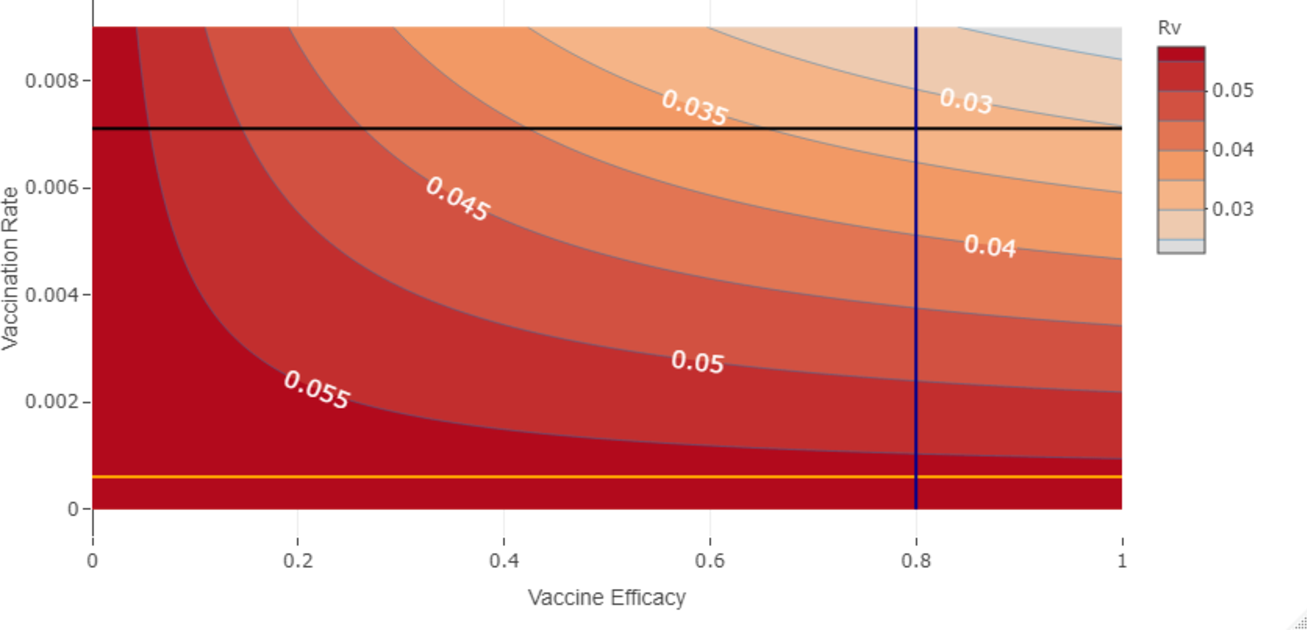
\includegraphics[scale=0.565, keepaspectratio]{Figures/Rv_contour}
    \caption{R not contour plot as function of efficacy and vaccination rate.}
    \label{fig:rvcontour1}
\end{figure*}

\begin{figure*}[tbh]
    \centering
    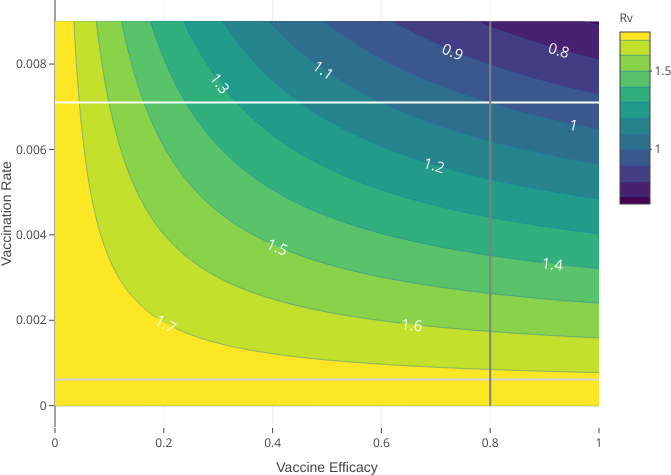
\includegraphics[scale=2.1, keepaspectratio]{Figures/R0_contour_1}
    \caption{R not contour plot as function of efficacy and vaccination rate.}
    \label{fig:r0contour1}
\end{figure*}


